%%%%
\documentclass[a4paper,11pt]{article}
%%%%
%%%%
%PACKAGES______________________________________________________________________________________
\usepackage{simplewick} %Allows Wick Notation
\usepackage{slashed} %Allows feynman slash notation 
\usepackage{graphicx} % graphics, pictures, figures
\usepackage{caption}
\usepackage{subcaption}
\usepackage{verbatim} % importing numerical scripts
\usepackage{multicol, float} % placing floats in right places
\usepackage{algpseudocode} % no idea...
\usepackage[utf8]{inputenc}
\usepackage{amssymb} %needed if not using mathdesign
\usepackage{amsmath}
\usepackage[OT1]{fontenc}
\usepackage{lmodern} %gfsartemisia, times, boisik, et cetera
\usepackage{braket} %dirac notation
\usepackage[cm]{fullpage} % for fulpage style
\usepackage{bm} % boldface vectors
\usepackage{float} % placing floats
\usepackage{relsize} % for \mathlarger command
\usepackage{mathrsfs} %?
\usepackage{textgreek} % cb-greek class
\usepackage{sectsty} % for centering sections
\usepackage{textcomp } % for nr. symbol
\usepackage[usenames, dvipsnames]{color} % defining own colors
\usepackage{type1cm} % scalable fonts
\usepackage{lettrine} % larger first letter in paragraph.
\usepackage{listings} % code-snippets in the text
\usepackage{background} % used for top page text
%\usepackage{niceframe} % for old-school double frame
\usepackage{tikz} % figure config/ creation
%\usepackage{bbold}
%\usepackage{swrule} % for fancy line
%\usepackage{pdfpages} % for importing pdf

%%%%
%%%% SET-UP NEEDED FOR FURTHER PACKAGES
%%%%
\definecolor{hyperclrblue}{RGB}{30,90,125} %Definind own color ; blue
\definecolor{hyperclrorng}{RGB}{210,100,45}%Definind own color
\definecolor{hyperclrgreen}{RGB}{60,120,20}%Definind own color
\usepackage[colorlinks = true,
linkcolor = hyperclrblue,
urlcolor = blue,
citecolor = blue,
anchorcolor = blue]{hyperref} % link package
\usepackage{pgfplots} % to plot directly into latex
\pgfplotsset{compat=1.5} % needed forpgfplots
\usepackage{framed, color} % for framing/shaded box
\definecolor{shadecolor}{cmyk}{0,0,0.185,0} % color for shaded box
\usepackage{fancybox}
\usepackage[sc]{titlesec} % title package
%_______________________________________________________________________________________________
%NEW COMMANDS_________________________________________________________________________________
%\renewcommand*{\thefootnote}{$\dagger$} % creating dagger footnote
\newcommand*{\boisik}{\fontfamily{bsk}\selectfont} % change font to boisik command
\newcommand{\wf}{\text{\textpsi}} % defining wavefunctions as cbgreek class.
\newcommand{\bwf}{\text{\textPsi}} % defining Wavefunctions as cbgreek class.
\newcommand{\Q}{\hat{\text{\boisik Q}}} % defining operator-style 'Q'
\newcommand{\nlm}{\ket{n\ell m_\ell}} % defining wavefunctions as cbgreek class.
\newcommand{\nlmz}{\ket{n\ell m_\ell;0}} % defining wavefunctions as cbgreek class.
\newcommand{\nlmt}{\ket{n\ell m_\ell;t}} % defining wavefunctions as cbgreek class.
%_____________________________________________
%\numberwithin{equation}{section} %equations labeled by section
\sectionfont{\centering} % centering sections with 'sectsty'
\subsectionfont{\centering} % centering sections with 'sectsty'
\definecolor{myclr}{RGB}{190,90,20} %Definind own color
\renewcommand{\thesection}{\Roman{section}.} % Roman numerals for sections
\renewcommand{\thesubsection}{\Alph{subsection}} % Roman numerals for subsections
\titleformat{\section}{\large\scshape\centering}{\thesection}{1em}{} % Change the look of the section titles
\titleformat{\subsection}{\normalsize\centering\bfseries}{\thesubsection.}{1em}{} % Change the look of the section titles
\setlength{\columnsep}{0.7cm}
%______________________________________________________________________________________________
%%%%
%%%%_________________________________________________________________________________________
\begin{document}
%%%% TOP PAGE TEXT
{\SetBgContents{ \textit{{\small\textsc{ Ask J. Markestad, Thorbjørn V. Larsen Universitetet i Oslo. \hspace{3.5cm} \textit{\today}}}}}
\SetBgScale{1}
\SetBgColor{black}
\SetBgAngle{0}
\SetBgOpacity{1}
\SetBgPosition{current page.north east}
\SetBgVshift{-1.2cm}
\SetBgHshift{-10.5cm}
%%%% CREATING TITLE HEADER
$$\:$$
\begin{center}
	\vspace{0.2cm}%\boisik
	\fontsize{15}{15}\selectfont \textsc{ Project 1: Vector and Matrix Operations in c++},\\
	%{in}}\\
	\fontsize{13}{13}\selectfont \textsc{Fys $\textnormal{{4150}}$ }\\
	\vspace{0.4cm}
	\fontsize{12}{12}\selectfont {\textsc{ Ask J. Markestad, Thorbjørn V. Larsen }}\\
	\vspace{0.5cm}
\end{center}
%%%%
%%%%
%______________________________________________________________________________________________
%%%%
%%%%
	
%\includegraphics[scale = 0.48]{line}
\rule{\textwidth}{0.3pt}\par
		
%---------------------------------------------------------------------------------------------------------------------------------------
\begin{abstract}
	We study the Gaussian elimination method for solving a linearized second order inhomogeneous differential equation over an interval with Dirichlet boundary conditions, using both a general Gaussian elimination method for tridiagonal matrix and one tailored for our three point approximation to the second derivative and compare their speed. We also use preexisting packages, armadillo, to solve the same problem by LU-decomposition to show the difference in calculation time between a general, always applicable method and our problem specific method.
\end{abstract}



		
\section*{Introduction}
		
Differential equations are fundamental in physics. The standard approach in most branches of physics is to describe a physical system in terms of it's symmetries and degrees of freedom through the formalism of Lagrange or Hamilton, i.e. by setting up equations of motion. It is thus a very important tool to be able to solve these differential equations as precisely and effectively as possible. In this project we explore algorithms for calculating second order differential equations using vector and matrix operations with the aim to better understand the computational demands of differential equation solutions and how to reduce these demands. Using the three point derivative approximation for the second order derivative we find that the matrix representing out set of coupled differential equations is a tridiagonal one. We use the Gaussian elimination method of forward and backward substitution to diagonalize this matrix for general matrix elements. We test the accuracy of this method with increasing number of points. The next step is then to use our specific form of our symmetric tridiagonal matrix with only three unique elements to create an even faster algorithm, allowing us to compare their speed difference. Finally we use the LU-decomposition method to solve our matrix equation. To do this we use already preexisting efficient code from the armadillo package, and then compare computational speed of this method for solving general matrix equations to our specialized algorithm.
		
		
		
\section*{Theory and Algorithms}
		
The following Gaussian elimination method for tridiagonal matrices is taken in large part from Computational Physics Lecture Notes Fall 2015 by Morten Hjort-Jensen \cite{M.Hjort-Jensen_CompFys}. We will be looking in detail at linear second-order differential equations.
		
$$\frac{d^2y}{dx^2} + k^2(x) y = f(x)$$
		
More specifically, we will look at differential equations where $k^2(x) = 0$. A known physics example of this type of equation would be Poisson's equation in radial coordinates for spherically symmetric source term.
		
$$\frac{d^2 \phi}{d r^2} = f(r)$$
		
In Newtonian gravity or in electromagnetism the source term is associated with a charge or mass distribution with a negative sign to explicitly indicate the attractiveness of the resulting potential. We will therefore look closely at the equation:
		
\begin{equation}
	- u''(x) = f(x)
	\label{diff_eq}
\end{equation}
	
With Dirichlet boundary conditions, i.e. $ x \in (0,1), \: \: u(0) = u(1) = 0$. To solve this equation numerically we need to discretize the functions $u$ and $f$ with grid points $x_i = i h$ from 0 to 1 in $n+1$ steps using step length $h = 1/(n+1)$. This means that we know the initial and final point of $u$ through the boundary conditions, and that we can use the three point derivative formula to rewrite the equation as:
		
\begin{equation}
	- \frac{u_{i+1} - 2u_i + u_{i-1}}{h^2} = f_i \: \: \: \: \: \: \: \: \text{for} \: \: i = 1, 2, ... , n
	\label{disc_diff_eq}
\end{equation}
		
The solution to this equation with the given boundary conditions is: 
\begin{equation}
u(x) = 1 - (1-e^{-10}) - e^{-10x}
\label{exact_solution}
\end{equation}

For $x = 0$ we get $u(0) = 1 - (1 - e^{-10})*0 - e^{-10 * 0} = 1-1 = 0$, and for $x = 1$ we get $u(1) = 1 - 1 + e^{-10} - e^{-10} = 0$, so it satisfies the boundary conditions and by deriving it twice we get $u'(x) = -(1-e^{-10}) + 10e^{-10x}, \: \: \: u''(x) = -100 e^{-10x}$. So we have found the exact solution to the differential equation which gives us a value to compare to, to see the accuracy of our numerical method. The next step to solve the equation is to rewrite it as a linear set of equations:
		
\begin{equation}
\begin{pmatrix}
	2 & -1 & 0 & ... & ... & 0 \\
	-1 & 2 & -1 & 0 & ... & 0 \\
	0 & -1 & 2 & -1 & 0 & ... \\
	... & ... & ... & ... & ... & ... \\
	0 & ... & 0 & -1 & 2 & -1 \\
	0 & 0 & ... & 0 & -1 & 2 
	\end{pmatrix} \begin{pmatrix}
	u_1\\
	u_2\\
	u_3\\
	...\\
	...\\
	u_n
	\end{pmatrix} = \begin{pmatrix}
	f_1 h^2 \\
	f_2 h^2 \\
	f_3 h^2 \\
	... \\
	... \\
	f_n h^2 \\
	\end{pmatrix}
\end{equation}
		
From here on out we will absorb the $h^2$ term into the source function. We will now take a step back and look at a more general matrix $\mathbf{A}$ for this sort of linear problem and developing an algorithm for it. This allows us to see the difference in CPU time between the general algorithm and one made specifically for our very symmetric case. The more general matrix we will look at is a tridiagonal matrix:
		
\begin{equation}
\mathbf{A} = \begin{pmatrix}
b_1 & c_1 & 0 & ... & ... & 0 \\
a_1 & b_2 & c_2 & 0 & ... & 0 \\
0 & a_2 & b_3 & c_3 & 0 & ... \\
... & ... & ... & ... & ... & ... \\
0 & ... & 0 & a_{n-2} & b_{n-1} & c_{n-1} \\
0 & 0 & ... & 0 & a_{n-1} & b_{n} 
\end{pmatrix}
\label{general_tridiagonal_matrix}
\end{equation}
		
		\subsection{General solver}
We now see that this problem is on the type $\mathbf{A}\mathbf{u}=\mathbf{f}$ were we know the values of $\mathbf{A}$ and $\mathbf{f}$. A solution for this problem is to form a diagonal matrix of $\mathbf{A}$, such that we easily can read out the values of $\mathbf{u}$. As the matrix is tridiagonal we can do this in two steps, forward-substitution where we remove the $a$ values and backward-substitution were we remove the $c$ values. Looking at the first 2 rows, we see that if we subtract the first row multiplied by $a_1/b_1$ we get
		
\begin{equation}
\begin{pmatrix}
b_1 & c_1 & 0 & ... & ... & 0 \\
0 & b_2-\frac{a_1 c_1}{b_1} & c_2 & 0 & ... & 0 \\
0 & a_2 & b_3 & c_3 & 0 & ... \\
... & ... & ... & ... & ... & ... \\
0 & ... & 0 & a_{n-2} & b_{n-1} & c_{n-1} \\
0 & 0 & ... & 0 & a_{n-1} & b_{n} 
\end{pmatrix} \begin{pmatrix}
u_1\\
u_2\\
u_3\\
...\\
...\\
u_n
\end{pmatrix} = \begin{pmatrix}
f_1 \\
f_2-\frac{f_1 a_1}{b_1} \\
f_3 \\
... \\
... \\
f_n \\
\end{pmatrix}
\end{equation}
		
If we do this all the way to the end of the matrix, we get a new matrix with only non-zero elements on and above the diagonal. If we call the new values of the diagonal element $\tilde{b}$ we have an explicit expression for them as
		
\begin{equation}
\tilde{b_i}=b_{i}-\frac{a_{i-1}c_{i-1}}{\tilde{b_{i-1}}}\quad i = 2, ..., n
\label{eq:forward_general_b}
\end{equation}
We also have to update the $\mathbf{f}$ in a similar manner
\begin{equation}
\tilde{f_i}=f_{i}-\frac{a_{i-1}f_{i-1}}{\tilde{b_{i-1}}}\quad i = 2, ..., n
\label{eq:forward_general_f}
\end{equation}
		
In the end of the forward substitution we have
		
\begin{equation}
\begin{pmatrix}
b_1 & c_1 & 0 & ... & ... & 0 \\
0 & \tilde{b_2} & c_2 & 0 & ... & 0 \\
0 & 0 & \tilde{b_3} & c_3 & 0 & ... \\
... & ... & ... & ... & ... & ... \\
0 & ... & 0 & 0 & \tilde{b_{n-1}} & c_{n-1} \\
0 & 0 & ... & 0 & 0 & \tilde{b_{n}}
\end{pmatrix} \begin{pmatrix}
u_1\\
u_2\\
u_3\\
...\\
...\\
u_n
\end{pmatrix} = \begin{pmatrix}
f_1 \\
\tilde{f_2} \\
\tilde{f_3} \\
... \\
... \\
\tilde{f_n} \\
\end{pmatrix}
\end{equation}
		
To continue we have to remove the elements above the diagonal. This time we first look at the elements in the last row that the first elements $u_n$ is given by $\tilde{f_n}/\tilde{b_n}$. To find the next elements $u_{n-1}$ we simply see that the equation for this row is 
		
\begin{equation}
u_{n-1}\tilde{b_{n-1}}+c_{n-1}u_n = \tilde{f_{n-1}}
\end{equation}
		
We know all values except $u_{n-1}$ and solve for this value in an iterative process upwards. This gives the algorithm 
		
\begin{equation}
u_i = \frac{\tilde{f_i}-c_i u_{i+1}}{\tilde{b_i}}\quad i = n-1, n-2, ..., 1
\label{eq:forward_general_u}
\end{equation}
	
where the sequence for the i's are important(i.e starting with the known value in the bottom). If we count the flops without any further simplifications, we get $3*3n=9n$ flops. Later in the algorithm section we see that we can actually reduce this value by 1 to get 8n flops. 
		
		\subsection{Specialized solver}
We can then look at our specialized example were we know the coefficients of the matrix $\mathbf{A}$. By precalculation some of the algorithms we can reduce the number of operations for a given grid size n by a substantial factor. If we insert the numbers into the first forward substitution equation \ref{eq:forward_general_b} we get
		
\begin{equation}
\tilde{b_i}=2-\frac{1}{\tilde{b_{i-1}}}\quad i = 2, ..., n
\end{equation}
		
For n=2,3,4 we have 
		
\begin{align}
\tilde{b_2}=2-\frac{1}{2}=\frac{3}{2} \\
\tilde{b_3}=2-\frac{2}{3}=\frac{4}{3} \\
\tilde{b_4}=2-\frac{3}{4}=\frac{5}{4}
\end{align}
	
where we start to suspect a series on the form
		
\begin{equation}
\tilde{b_i}=\frac{i+1}{i}  \quad i = 2, ..., n
\label{eq:forward_specific_b}
\end{equation}
		
We can see that this step only has 2n flops, and will always contain the same elements. The equations for $\mathbf{f}$ also simplify to
\begin{equation}
\tilde{f_i}=f_{i}+\frac{f_{i-1}}{\tilde{b_{i-1}}}\quad i = 2, ..., n
\label{eq:forward_specific_f}
\end{equation}
		
where we now equally have 2n flops for this step. 
		
For the backward substitution we get 
		
\begin{equation}
u_i = \frac{\tilde{f_i} + u_{i+1}}{\tilde{b_i}}\quad i = n-1, n-2, ..., 1
\label{eq:forward_specific_u}
\end{equation}
		
which has 2n flops. 
This gives in total 6n flops for this specified algorithm, a significant improvement compared to the general case. 


LU decomposition is an efficient method for solving matrix equations for general matrices \cite{M.Hjort-Jensen_CompFys}, however for our matrix where most of the elements are zero it becomes very inefficient. To illustrate this point we will be using LU decomposition function and LU backwards algorithm from the armadillo package (Is included with our source code linked below). 

	
\subsection{Memory handling and algorithms}

Source code and accompanying codes can be found at the git hub address:

\url{https://github.com/ajmarkestad/Fys4150/tree/master/Project1} 



To efficiently handle the memory and not generate lots of copies of the matrices, vectors are used as the algorithms act on a vector-type structure. For each round of the general algorithm(as in the forward substitution of b) we can pass the array by reference and only update the values. The pseudocode for the forwards substitution would then be
\begin{lstlisting}
//general forward algorithm
for (int i=1; i<=n; i++)
	{
	b[i]=b[i]-c[i-1]*b[i-1]/b[i-1];
	f[i]=f[i]-c[i-1]*f[i-1]/b[i-1];
	}
\end{lstlisting}
		
We notice that the factor $a[i-1]/b[i-1]$ gets calculated twice. This is a waste of flops, so to reduce the number of flops by 1 we can calculate this value and save it as an intermediate step. This will now give

\begin{lstlisting}
//general forward algorithm
double intermediate; 
for (int i=1; i<=n; i++)
	{
	intermediate = a[i-1]/b[i-1];
	b[i]=b[i]-c[i-1]*intermediate;
	f[i]=f[i]-f[i-1]*intermediate;
	}
\end{lstlisting}
		
\begin{lstlisting}
//general backward algorithm
//start at 1 as the 0 elements is ok
for (int i=n-1; i>=0; i--)
	{
	u[i]=(f[i]+u[i+1])/b[i];
	}
\end{lstlisting}
		
We see that in total we have 8n flops for the general algorithm. We know that in a specialized case where we tailor the algorithm for the problem we usually can reduce the number of flops, so let's go through such a process for the specified program. Inserting the improvements we already have found, we get
		
\begin{lstlisting}
//specified forward algorithm
//start at 1 as the 0 elements is ok
for (int i=1; i<n; i++)
	{
	f[i]=f[i]+f[i-1]/pre_calculated[i-1];
	}
//specified backward algorithm
//start at 1 as the 0 elements is ok
for (int i=n-2; i>=0; i--)
	{
	u[i]=(f[i]+u[i+1])/pre_calculated[i-1];
	}
\end{lstlisting}
		
where the $pre\_ calculated$ variable is a list already filled before the algorithm(see equation \ref{eq:forward_specific_b} for the formula). By these improvements the algorithm will require of the order 4n flops, an $50\%$ reduction in computing time relative to the general solver. We will later see that other effects will come into play when comparing the actual time for computing, but these will nevertheless be around an $\frac{1}{2}$ reduction in CPU-time.  

\subsection{LU}
The LU-algorithm is based on storing and manipulating full matrices and will require in general the square of the memory required for our vectorized implementation. For grid sizes on the order of $10^4$ and higher this will require around 1 GB of memory, while for the vectors the needs are of the order 80 KB. To handle this problem we will not include LU-decomposition and solving for grid sizes larger than $10^3$ points. 

\section*{Results}

A comparison plot between the numerically computed solution to the differential equation and the exact solution \ref{exact_solution} is shown in figure \ref{fig:exact_vs_calculated} for grid sizes with 10, 100, and 1000 points. From a visual inspection we cannot distinguish the two function already for only 100 grid points. From table \ref*{table:Results} we see that the max relative error between the two functions is of the order $10^{-3}$ or 0.1 \% error. When increasing N we see that for $N>10^{5}$ grid points the accuracy decreases due to round off error when we subtract in the algorithm. Therefor, for most practical purposes we can keep the grid size in the 1000 point range to ensure a fast and accurate result without having to set aside a large amount of memory. On another note, for some applications a small error is extremely important. In such cases it is important to notice that until we hit the point where $log10(N)=5$, the memory and time used for the computation scales linearly with N, while the maximum error scales almost like $1/N^2$ which is a good trade-off. 



\begin{figure}[H]
	\centering
	\begin{subfigure}[b]{0.3\textwidth}
		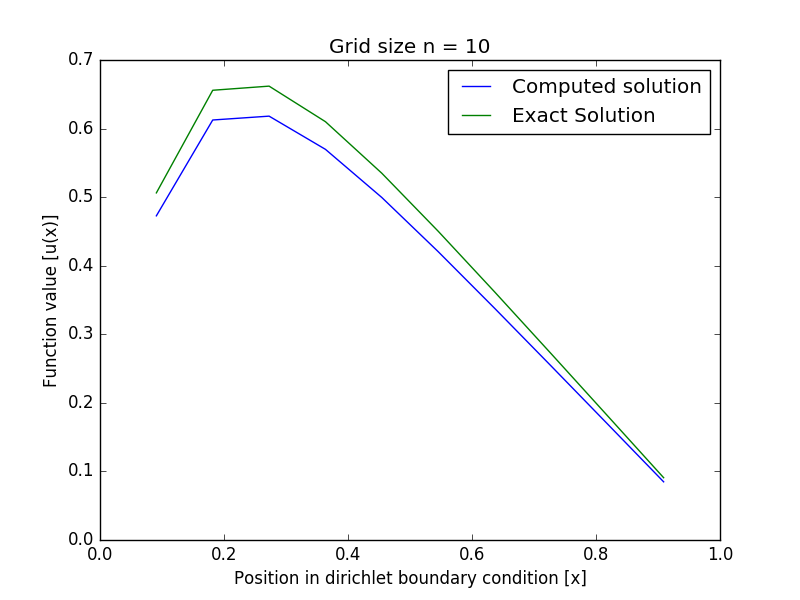
\includegraphics[scale=0.3]{n=10}
		\caption{Calculated using grid size n = 10}
		\label{fig:n=10}
	\end{subfigure}
	\begin{subfigure}[b]{0.3\textwidth}
		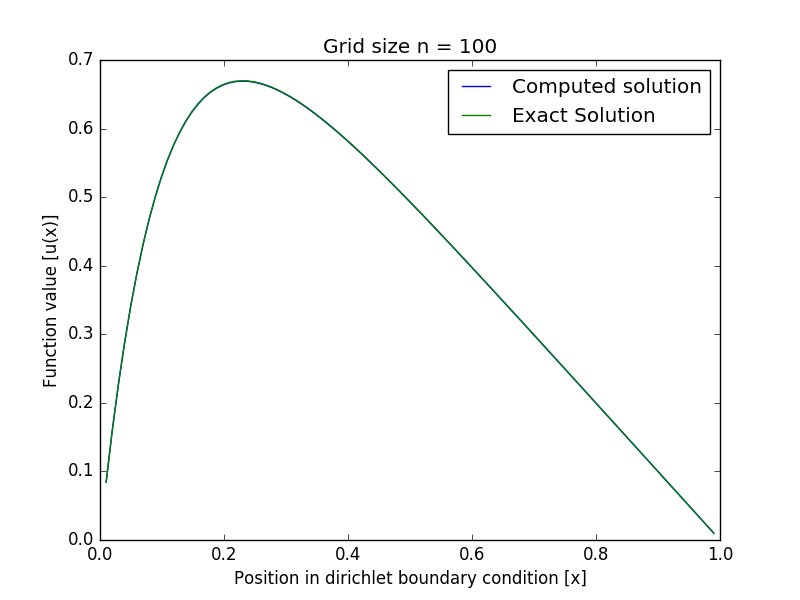
\includegraphics[scale=0.3]{n=100}
		\caption{Calculated using grid size n = 100}
		\label{fig:n=100}
	\end{subfigure}
	\begin{subfigure}[b]{0.3\textwidth}
		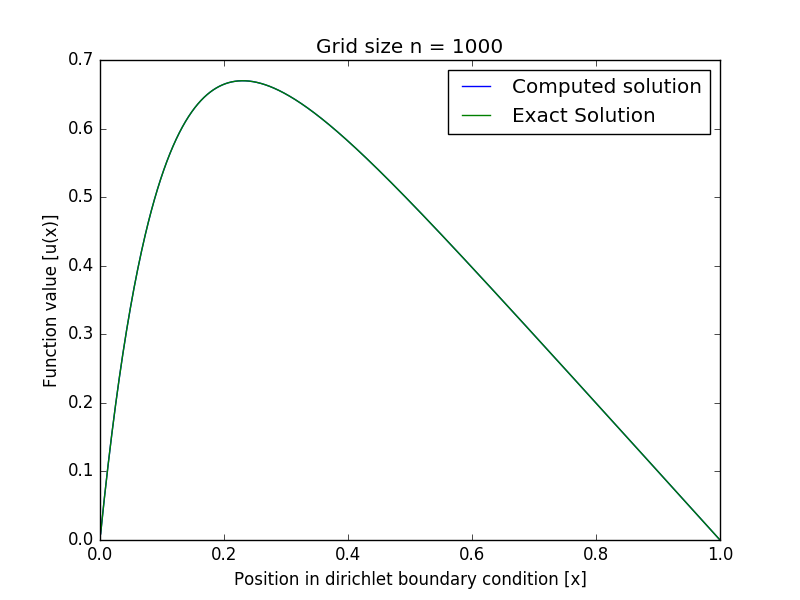
\includegraphics[scale=0.3]{n=1000}
		\caption{Calculated using grid size n = 100}
		\label{fig:n=1000}
	\end{subfigure}
	\caption{Comparison between the exact solution to the differential equation and the one computed using Gaussian elimination for a grid sizes of n = 10, 100, and 1000. Here the two points determined by the boundary condition is left out as they are known and are thus not calculated.}
	\label{fig:exact_vs_calculated}
\end{figure}

\begin{figure}
	\centering
	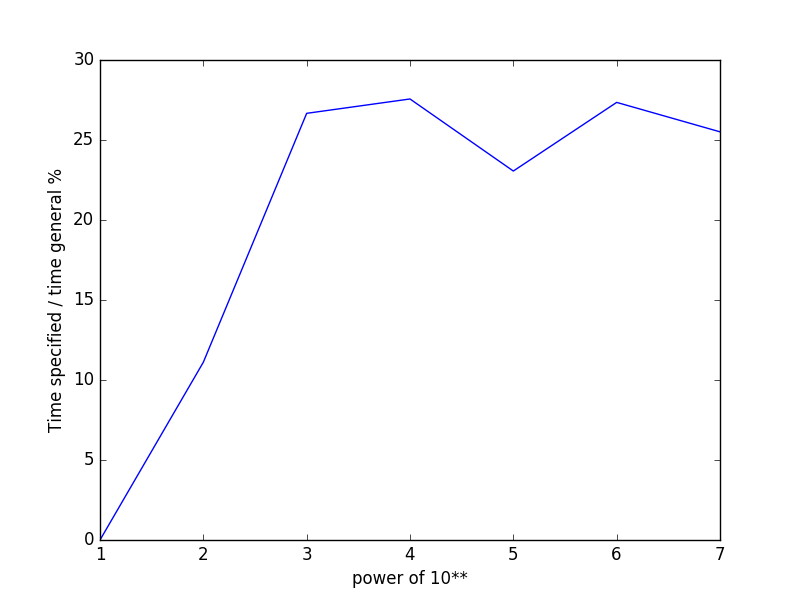
\includegraphics[scale=0.5]{Time_relative}
	\caption{Relative radio of the time spend on the specified algorithm to the general algorithm. For each power of 10 the average of 1000 runs was calculated and used for each algorithm. There is a pronounced leveling off as N increases, which could be interpreted as the overhead of calling a function becomes less important compared to the calculations}
	\label{fig:Time_relative}
\end{figure}

We can further compare run-times for the specialized vs general algorithm. This was done by for each grid size up to $10^7$ and in each loop the average of 1000 function calls was calculated. In figure \ref{fig:Time_relative} one can see that after increasing the grid size above $10^3$ the ratio of time spend by the algorithms is relatively stable. It levels off around a value of 0.35 which means we gain an even higher speedup compared to what we had expected from our simple counting of mathematical operations(4n vs 8n flops). A possible explanation for this effect is that all flops are not equal. A multiplication could take more time that a simple addition and with a different number of operation types for each algorithm this difference could leading to different performance. These is also an extra storing of an intermediate value in the general solver, which could lead to extra CPU-time. It is also interesting to note that for low grid sizes the ratio is even farther in favor of the specialized algorithm. We theorize that since for low values of n the time difference in the actual calculations is negligible and the time difference then emerges because of the different structures of the functions defined to do the calculations. Since the general solver has to take in more variables then the specialized solver, we suspect that it will take longer to run through. We therefore hypothesize a relation for the relative time:

\begin{equation}
\text{relative time} = \frac{\text{fixed time due to general solver function structure} + 8n}{\text{fixed time due to specialized solver function structure} + 4n}
\end{equation}

So for small n the CPU dominating process is the structure of the functions, but as n increases the ratio shifts until finally for sufficiently large n values it is the flop ratio that is the dominating factor.
		
\begin{table}[H]
	\centering
	\caption{The results of our accuracy and speed difference tests. The max relative error is calculated by comparison between the general tridiagonal Gaussian elimination method and the exact solution for grid sizes varying from n = 10 to n = $10^{7}$. The time specified in the table is the CPU time of the algorithm for general tridiagonal matrix, our specific tridiagonal matrix and using a general LU decomposition algorithm}
	\label{table:Results}
	\begin{tabular}{|lllll|} \hline
		log10(N) & log10($\epsilon$) & Time General (s)     & Time Special(s)      & Time LU(s) \\
		\hline 
		1        & $-1.359$       &$2.000\cdot 10^{-6}$  &$0.000$              &  $0.0001410$    \\
		2        & $-3.262$       &$9.000\cdot 10^{-6}$  &$1.000\cdot 10^{-6}$ &  $0.0007060$        \\
		3        & $-5.254$       &$1.500\cdot 10^{-5}$  &$4.000\cdot 10^{-6}$ &  $0.08217$      \\
		4        & $-7.253$       &$0.0001560$ 	         &$4.300\cdot 10^{-5}$ &   NA       \\
		5        & $-9.044$       &$0.001843$	         &$0.0004250$	       &   NA       \\
		6        & $-6.351$       &$0.01808$	         &$0.004945$	       &   NA       \\
		7 	     & $-6.199$		  &$0.1967$ 		     &$0.05018$ 		   &   NA \\
		\hline
	\end{tabular}
\end{table}


		
		
Going to the time spend on the LU-method we see that there in an enormous increase in time spent to compute as it scales with $\propto N^3$. If we had included $N=10^4$ this calculation alone would have taken in the order of a minute, and requiring 1 GB of memory. 

\section*{Conclusion}
		
In conclusion, with the tridiagonal Gaussian elimination method there is an upper limit of $10^{5}$ grid points due to round off errors occurring at higher grid point values. At this upper grid point limit the time ratio for the general tridiagonal algorithm to the specialized for our matrix is of the order 3. We see clearly that each method for solving the problem has it's advantages and disadvantages, considering CPU-time, memory requirement and generality. While the LU-method is a general method that can handle matrices that are not only tridiagonal, it quickly runs into hardware limitations giving a practical limitation in the accuracy of the solution(only up to $log10(max\_error)\propto -5$) For differential equations on the type given in the introduction, the specialized algorithm shown in this project was the best way to proceed. 
		
		
		
		
\begin{thebibliography}{3}
			
	\bibitem{M.Hjort-Jensen_CompFys}
	Morten Hjort-Jensen
	\emph{ Computational Physics Lecture Notes Fall 2015}
	Department of Physics, University of Oslo
	2015
	\url{https://github.com/CompPhysics/ComputationalPhysics/blob/master/doc/Lectures/lectures2015.pdf}
			
			
			
			
			
\end{thebibliography}
		
		
		
		
		
		
		
		
		
%__________________________________________________________________________
\end{document}